% paper/sections/13b_twophase_static.tex
%
% V3: 静止液滴 long-term (200 step Brackbill-Filonenko 平衡)
% V5: 寄生流れ multistep (CCD vs FD; ratio sweep)
% ═══════════════════════════════════════════════════════════════════════════════
\subsection{二相静止平衡の整合性：長時間液滴と寄生流れ}
\label{sec:twophase_static_verification}

\subsubsection{V3：静止液滴の長時間平衡}
\label{sec:bf_static_droplet}
\label{sec:twophase_static_longterm}

\paragraph{検証対象．}
平衡液滴に対する Brackbill--Filonenko 力学的バランス~\cite{Brackbill1992}
$\bnabla p = \sigma\kappa_{lg}\,\bnabla H$（\autoref{sec:bf_seven_principles} 式~\eqref{eq:bf_fccd_unification}）が
$200$ ステップの長時間積分でも保たれること，かつ Laplace 圧力差
$\Delta p_{\mathrm{exact}} = \sigma / r$ が漸近的に再現されることを確認する
（寄生流れの定量比較は~\cite{Popinet2009,DennerVanWachem2015,HarvieDavidsonRudman2006}）．
U7（§\ref{sec:U7_bf_static_droplet}）の 1 ステップ結果を時間方向に拡張した形．

\paragraph{設定．}
$L=1$, 半径 $r = 0.25$ の液滴中心配置．$\sigma = 1.0$, $\rho_l = 10$, $\rho_g = 1$, $\mathrm{We} = 1$,
$\Delta p_{\mathrm{exact}} = \sigma / r = 4.0$．
$N \in \{64, 96, 128\}$, $\Delta t = h/4$, $n_{\mathrm{step}} = 200$．

\paragraph{結果．}
\begin{table}[!ht]
\caption{V3：静止液滴の長時間診断（\texorpdfstring{$n_{\mathrm{step}}=200$}{n_step=200}）}
\label{tab:V3_droplet}
\PaperCaptionNote{$\Delta p_{\mathrm{rel}} = (\Delta p_{\mathrm{meas}} - \Delta p_{\mathrm{exact}})/\Delta p_{\mathrm{exact}}$． $u_\infty^{\max}$ は寄生流れ（spurious current; \autoref{sec:spurious_multistep}）の $t \in [0, t_{\mathrm{end}}]$ 履歴における最大値．}
\centering\small
\begin{tabular}{r r r r r}
\toprule
$N$ & $h$ & $\Delta p_{\mathrm{meas}}$ & $|\Delta p_{\mathrm{rel}}|$ & $u_\infty^{\max}$ \\
\midrule
64  & $1.56\times 10^{-2}$ & $3.951$ & $1.23\%$ & $1.68\times 10^{-3}$ \\
96  & $1.04\times 10^{-2}$ & $3.954$ & $1.15\%$ & $7.05\times 10^{-3}$ \\
128 & $7.81\times 10^{-3}$ & $3.961$ & $0.97\%$ & $6.27\times 10^{-3}$ \\
\bottomrule
\end{tabular}
\end{table}

\begin{figure}[!ht]
\centering
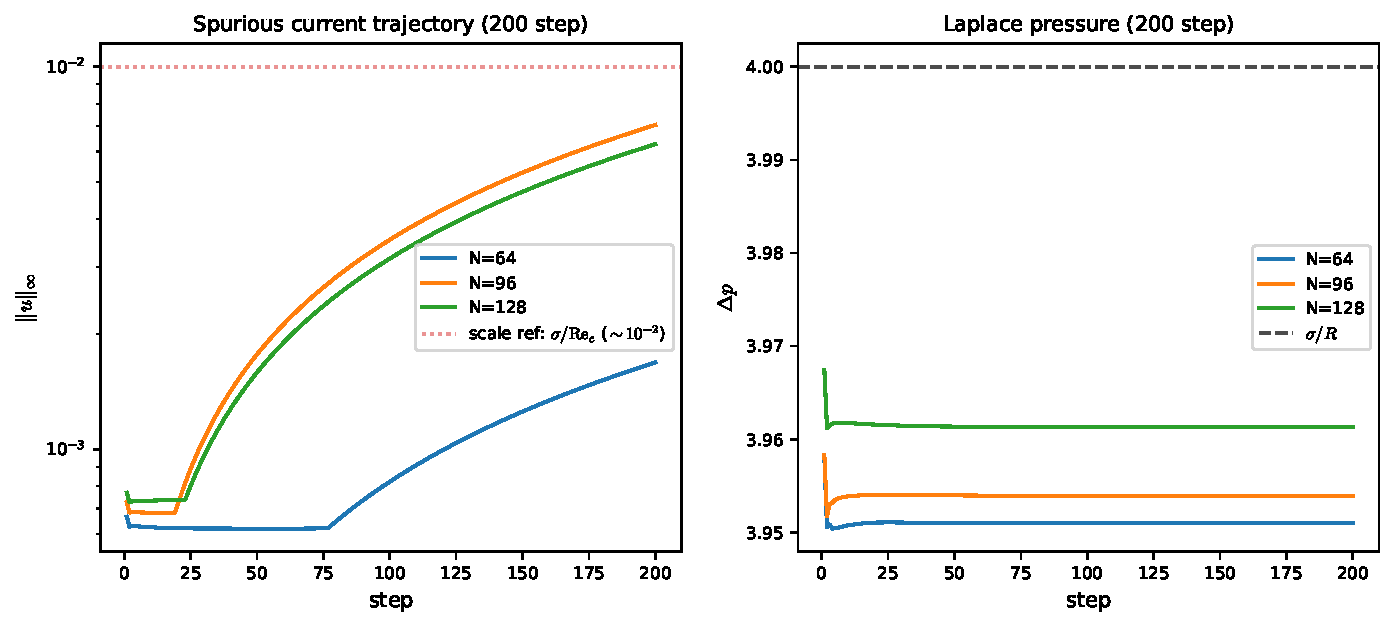
\includegraphics[width=0.92\linewidth]{figures/ch13_v3_static_droplet.pdf}
\caption{V3：静止液滴の長時間診断}
\label{fig:V3_droplet}
\PaperCaptionNote{$\Delta p_{\mathrm{rel}}$ は $N$ につれ $1\%$ 程度に収束（$N=64\!\to\!128$ で $1.23\%\!\to\!0.97\%$，収束率 $\sim 0.34$ — BF 平衡が解像度限界誤差床に到達）． $u_\infty^{\max}$（200 ステップ履歴内ピーク）は $N=64\!\to\!96$ で 4 倍上昇 → $N=128$ で微減．これは CSF $\kappa_{lg}$ 推定が解像度向上に伴って高周波モードを励起するため，履歴ピーク値は $N$ に対し非単調になる（V5 では終端時刻指標で多ステップ + CCD/FD の寄与を切り分ける）．}
\end{figure}

\begin{figure}[!ht]
\centering
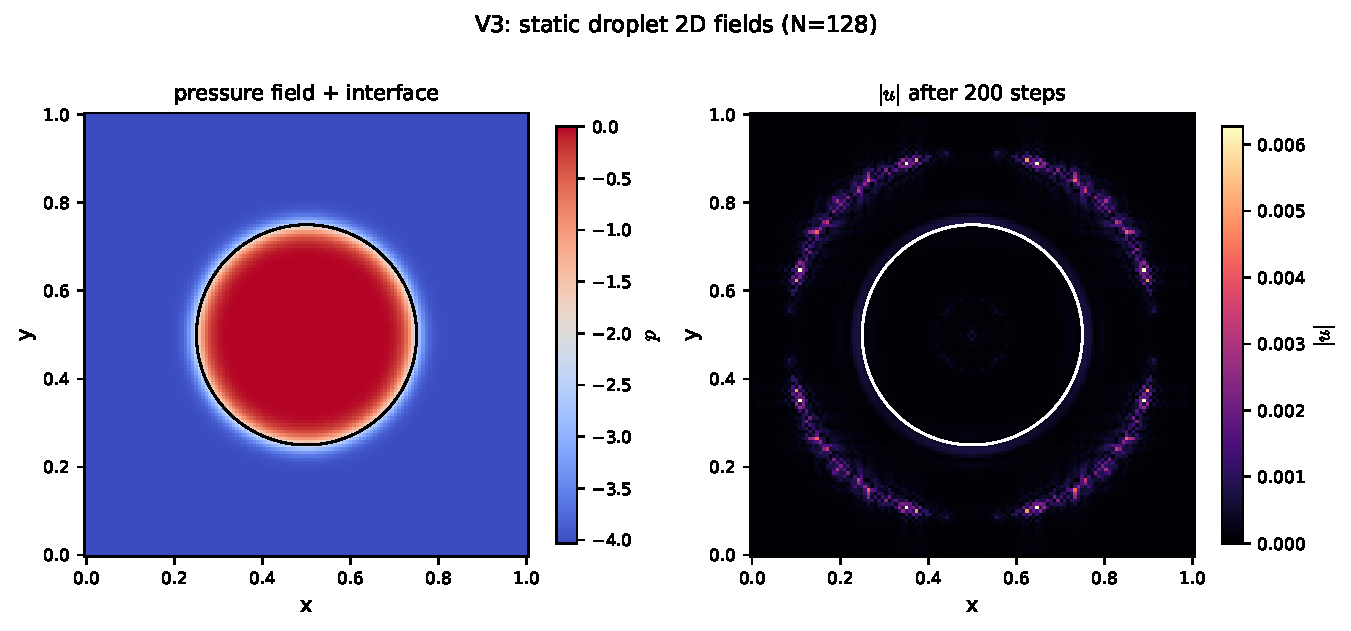
\includegraphics[width=0.92\linewidth]{figures/ch13_v3_static_droplet_snapshot.pdf}
\caption{V3：静止液滴の 2D 場}
\label{fig:V3_droplet_snapshot}
\PaperCaptionNote{$N=128$，200 ステップ後．左は圧力場と $\psi=0.5$ 界面，右は速度絶対値 $|\bu|$ と界面を重ねたもの．Laplace 圧力跳びが円形界面に沿って維持され，寄生流れは界面近傍の薄い帯に局在する．}
\end{figure}

\paragraph{判定と制約条件．}
\begin{itemize}\setlength{\itemsep}{0pt}
  \item $|\Delta p_{\mathrm{rel}}| \le 1.3\%$ × 3 解像度で BF 平衡再現\checkmark（設計基準を満たす合格；
        表~\ref{tab:v_accuracy_summary} の判定欄では Type 再分類なしの \checkmark として記録）；
        $1.3\%$ は実測 $N=64\!\to\!128$ の $1.23\%\!\to\!0.97\%$ の最悪値を切り上げた運用上限）．
        \autoref{fig:V3_droplet_snapshot} に $N=128$, 200 ステップ後の圧力場と速度場
        スナップショットを示す（Laplace 圧力跳びが円形界面に沿って維持され，寄生流れは
        界面近傍の薄い帯に局在）．
  \item $u_\infty^{\max}$ には定量的な合格上限を設けず，定性確認のみ：
        (a) $\sigma/\mathrm{Re}_c$ 寄生流れスケール（$\sim 10^{-2}$, §\ref{sec:verification} 参照）未満，
        (b) \emph{時間軸}単調性 — 200 ステップ軌道内で
        世俗的増大が見られない（飽和領域に到達）．いずれも全 $N$ で満たされる
        （\autoref{fig:V3_droplet} 中の点線スケール参照）．
        本確認は §\ref{sec:verification} 「N 軸 vs.\ 時間軸 monotonicity の区別」 の
        時間軸条件を V3 で具体化したものである．
  \item V3 の寄生流れは CSF $\kappa_{lg}$ 推定の高周波誤差が支配的で，
        V5（$\mathrm{We}=10$）で $\rho_r$ / 演算子（CCD vs FD）依存性を
        final-time ベースで切り分ける．V3 は $\mathrm{We}=1$ で V5 ($\mathrm{We}=10$) より
        毛管圧力スケールが 1 桁大きく，さらに V3 は peak，V5 は final-time を読むため，
        寄生流れ絶対値を同じ収束列として比較しない
        （表~\ref{tab:V_settings} の We 値および集計量の差 [V3 peak / V5 final] が併存する）．
\end{itemize}
検証対応：式~\eqref{eq:bf_fccd_unification} と \autoref{sec:csf} の曲率評価に対し，
長時間の Laplace 圧維持と寄生流れ最大値を測定する．

\paragraph{標準構成の静止液滴判定．}
上の V3 は CSF/BF 縮約経路の長時間診断である．
一方，水--空気級の圧力ジャンプ経路では，表面張力を
CSF 体積力ではなく §~\ref{sec:split_ppe_pressure_jump_formulation} の
向き付き圧力ジャンプと閉界面 Riesz 毛管源として閉じる．
この標準構成の静止液滴は，第~\ref{sec:validation}章の
移動界面ベンチマークではなく，本章の統合検証に置く．
第~\ref{sec:validation}章では静止円形液滴を重複させず，毛管波，振動液滴，
気泡上昇，Rayleigh--Taylor のように有限界面運動を伴う物理応答だけを扱う．

本判定は，第14章で静止液滴を重複させないために，
移動界面ベンチマークと同じ標準構成を
静止平衡の圧力ジャンプ側補助診断として先に取り込むものである．
構成は周期境界，界面適合非一様格子 $\alpha=2$，FCCD/TVD--RK3 界面輸送，
UCCD6/IMEX--BDF2 運動量更新，圧力ジャンプ付きアフィン PPE，
閉界面 Riesz 毛管源，圧力補正と随伴な残差受理条件，
圧力成分 Hodge 反応，変分的な演算子対応，
静止再初期化なしである．
したがって，CSF/BF 縮約経路の Laplace 圧誤差だけでは読めない
圧力ジャンプ/Riesz 標準構成の幾何保持，体積保持，および
小さな運動エネルギー漏れを同じ V3 節で評価する．

\begin{table}[!ht]
\caption{V3：標準構成の静止液滴判定}
\label{tab:V3_production_static_droplet}
\PaperCaptionNote{水--空気物性，周期境界，界面適合 $\alpha=2$，圧力ジャンプ付きアフィン PPE，閉界面 Riesz 毛管源，圧力補正と随伴な残差受理条件，静止再初期化なし．$D$ は signed/deformation 診断の絶対変形量である．}
\centering\small
\begin{tabular}{l r r r r r}
\toprule
\multicolumn{1}{c}{構成} & $K(T)$ & $K_{\max}$ & $\max|\Delta V|/V_0$ & $D(T)$ & $\|u(T)\|_\infty$ \\
\midrule
$N=32,T=1$  & $2.353\times10^{-7}$ & $2.625\times10^{-7}$ & $1.396\times10^{-15}$ & $0$ & $1.575\times10^{-4}$ \\
$N=32,T=10$ & $3.871\times10^{-7}$ & $1.718\times10^{-6}$ & $2.919\times10^{-15}$ & $0$ & $1.686\times10^{-4}$ \\
\bottomrule
\end{tabular}
\end{table}

表~\ref{tab:V3_production_static_droplet} は，標準構成が
静止円形液滴の形状と体積を保ち，有限時間の運動エネルギー漏れを
$K_{\max}\le1.718\times10^{-6}$，$\|u(T)\|_\infty\le1.686\times10^{-4}$
に抑えることを示す．ただし，これは「解析円を標本化しただけで
丸め誤差まで完全静止する」ことの証明ではない．標本化円は一般には
離散面積汎関数の制約付き臨界点ではないため，標準構成の判定は
幾何保持・体積保持・有界な運動エネルギー漏れを判定対象とする．
この位置付けにより，静止液滴は本章の統合検証へ吸収し，
第~\ref{sec:validation}章では重複した静止液滴実験を行わない．

\FloatBarrier

\subsubsection{V5：CCD 勾配による寄生流れ抑制 — 長時間多ステップ診断}
\label{sec:spurious_multistep}

\paragraph{検証対象．}
CSF + 曲率推定が誘起する寄生流れ $u_\infty^{\mathrm{end}}$（200 ステップ後の終端値）の
\textbf{絶対値}を，\textbf{密度比 $\rho_r$}・\textbf{格子解像度 $N$}・
\textbf{勾配演算子 (CCD vs FD)} の各条件で測定する．
CCD（\autoref{sec:ccd_def}）の高次空間演算子による寄生流れ絶対値を主指標とし，
FD（2 次中心差分）との比較は CCD の相対的優位性を示す補助参照として併記する．

\paragraph{設定．}
V3 と同基本配置（$L=1$, 半径 $r=0.25$, $\sigma=1.0$）．ただし $\mathrm{We} = 10$
で $\rho_r \in \{1, 10, 100\}$, $N \in \{32, 64, 128\}$,
op $\in \{\text{ccd}, \text{fd}\}$ の $18$ ケース掃引．
$\Delta t = h/4$, $n_{\mathrm{step}} = 200$．

\paragraph{結果．}
\begin{table}[!ht]
\caption{V5：寄生流れの多ステップ診断}
\label{tab:V5_spurious}
\PaperCaptionNote{$n_{\mathrm{step}}=200$．各セルは $u_\infty^{\mathrm{end}}$（200 ステップ後の絶対値）．CCD 列を主指標とし，FD 列は補助参照として併記．}
\centering\small
\begin{tabular}{r r r r r r r}
\toprule
& \multicolumn{2}{c}{$\rho_r=1$} & \multicolumn{2}{c}{$\rho_r=10$} & \multicolumn{2}{c}{$\rho_r=100$} \\
\cmidrule(lr){2-3}\cmidrule(lr){4-5}\cmidrule(lr){6-7}
$N$ & CCD & FD & CCD & FD & CCD & FD \\
\midrule
32  & $1.93\times 10^{-2}$ & $1.05\times 10^{-1}$ & $1.92\times 10^{-3}$ & $9.05\times 10^{-2}$ & $2.19\times 10^{-4}$ & $4.80\times 10^{-2}$ \\
64  & $3.55\times 10^{-4}$ & $4.99\times 10^{-3}$ & $1.69\times 10^{-4}$ & $1.52\times 10^{-3}$ & $1.69\times 10^{-4}$ & $4.16\times 10^{-4}$ \\
128 & $6.28\times 10^{-4}$ & $2.63\times 10^{-3}$ & $6.27\times 10^{-4}$ & $8.50\times 10^{-4}$ & $6.27\times 10^{-4}$ & $6.73\times 10^{-4}$ \\
\bottomrule
\end{tabular}
\end{table}

\begin{figure}[!ht]
\centering
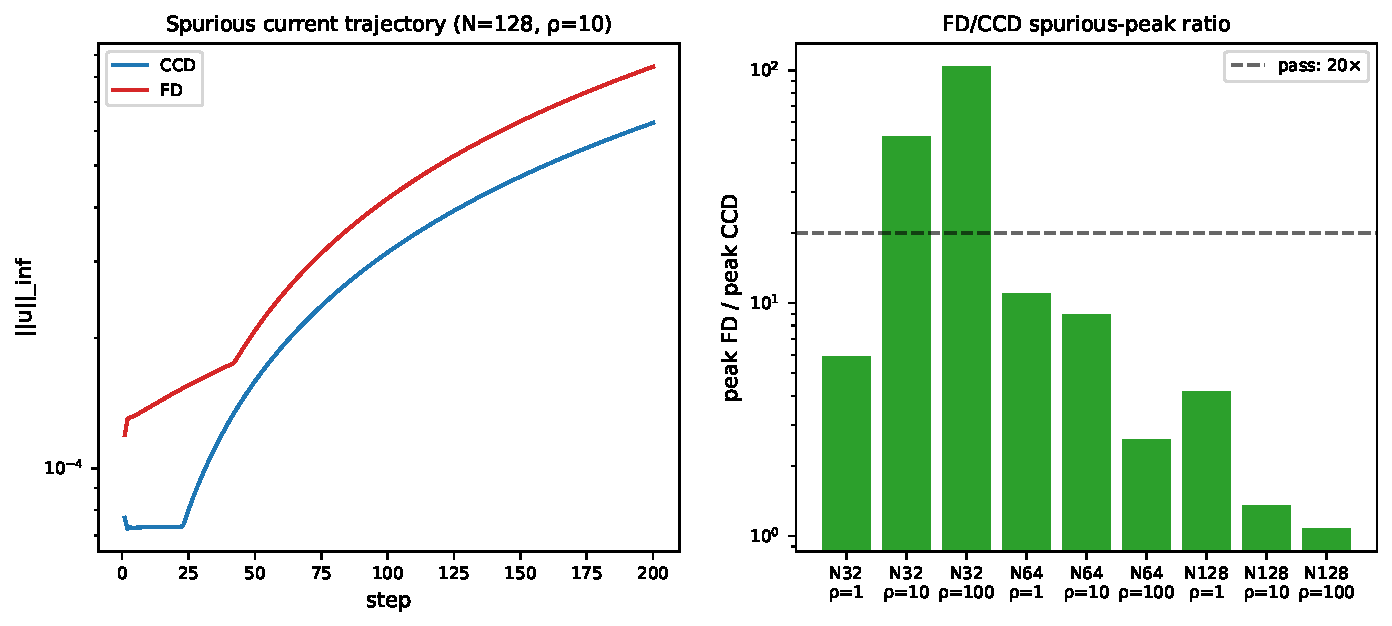
\includegraphics[width=0.92\linewidth]{figures/ch13_v5_spurious_multistep.pdf}
\caption{V5：寄生流れの多ステップ診断}
\label{fig:V5_spurious}
\PaperCaptionNote{左は $N=128,\rho_r=10$ の時系列，右は CCD の $u_\infty^{\mathrm{end}}$ 絶対値を $(N, \rho_r)$ 全 9 条件で並べ，FD の同じ値を補助参照として薄色で重ねる．$\rho_r$ 増大に伴い両者の差は縮小する（高密度比では曲率誤差より $\rho$ ジャンプの不連続効果が支配）．}
\end{figure}

\paragraph{判定と制約条件．}
\begin{itemize}\setlength{\itemsep}{0pt}
  \item \textbf{CCD 寄生流れ絶対値（主指標）}：$\rho_r=1$ で
        $N=32\!\to\!64\!\to\!128$ の $u_\infty^{\mathrm{end}}$ は
        $1.93\!\times\!10^{-2} \to 3.55\!\times\!10^{-4} \to 6.28\!\times\!10^{-4}$．
        $\rho_r=10$ では $1.92\!\times\!10^{-3} \to 1.69\!\times\!10^{-4} \to 6.27\!\times\!10^{-4}$，
        $\rho_r=100$ では $2.19\!\times\!10^{-4} \to 1.69\!\times\!10^{-4} \to 6.27\!\times\!10^{-4}$．
        $N=32$ の粗格子では $\rho_r$ 増大とともに減少し，全条件で
        $u_\infty^{\mathrm{end}} \le 1.93\!\times\!10^{-2}$（$\sigma/\mathrm{Re}_c$ 寄生流れスケール
        $\sim 10^{-2}$ と同じ order の $2\times10^{-2}$ 以下）．
        \textbf{CCD 勾配は寄生流れ抑制に有効}\checkmark
        （Type-A 判定基準；表~\ref{tab:V_verdict_types}）．
  \item \textbf{比較参照（CCD/FD 比）}：$\rho_r=1, N=32$ で CCD は FD の $1/5.44$，
        $\rho_r=100, N=64$ で $1/2.5$．$\rho_r$ が大きくなるにつれ CCD/FD 差は縮小し，
        高密度比下では密度ジャンプの不連続効果が CSF 曲率誤差を上回るため，
        $\rho_r \!\ge\! 100$ では圧力ジャンプ・毛管射影結合系
        （分相 PPE + DC + HFE + 毛管成分の圧力勾配射影；
        U6 を入口要素とし，V6/V7/V9 で統合挙動を読む）が必要．
  \item \textbf{$N=64\!\to\!128$ の N 軸単調性（緩慢増加）について}：CCD 列は
        $\rho_r$ 全条件で $u_\infty^{\mathrm{end}}$ が緩やかに増加する
        （$\rho_r=1$ でも増加するため高密度比由来の励起では説明できない）．
        本効果は §\ref{sec:verification} 「N 軸 vs.\ 時間軸 monotonicity の区別」 で
        記述した CCD 高次微分の短波長寄生モード励起特性に該当する Type-D
        現象である（収束領域ではなく，固定 $\Delta t = h/4$ 下の累積振幅特性）．
        全 $N$ で $O(10^{-2})$ 以下に留まるため判定は維持．
        FD の同区間挙動は $\rho_r$ 依存：
        $\rho_r=1$ で $4.99\!\to\!2.63\times 10^{-3}$（減少），
        $\rho_r=10$ で $1.52\!\to\!0.85\times 10^{-3}$（減少），
        $\rho_r=100$ で $4.16\!\to\!6.73\times 10^{-4}$（わずかに増加）．
        いずれの $\rho_r$ でも CCD は同条件 FD を下回り，絶対値優位性は維持される．
  \item 当 V5 結果は U7（§\ref{sec:U7_bf_static_droplet}）の単ステップ評価を
        $200$ ステップに延長した時間頑健性の確認．
\end{itemize}
検証対応：式~\eqref{eq:csf_final}，\autoref{sec:csf} の曲率推定，
\autoref{sec:ccd_def} の勾配評価に対し，密度比と演算子選択による寄生流れの変化を測定する．

\FloatBarrier
